\chapter{Tracce d'esame svolte - 2023}

\section{Esame del 16 gennaio 2023}
\begin{center}
	\includegraphics[scale=.85]{pdf/23-01-16.pdf}
\end{center}
\subsection*{Esercizio 1}
La tautologia della negazione dell'implicazione afferma che sono equivalenti le seguenti proposizioni:
\begin{align*}
	\neg(\alpha \implies \beta) \iff (\alpha \land \neg \beta)
\end{align*}
Infatti, sfruttando la tautologia dell'implicazione come disgiunzione abbiamo:
\begin{align*}
	\neg \bigl(\alpha \implies \beta \bigr) &\iff \neg \bigl( \neg \alpha \lor \beta \bigr) \\
	&\iff \neg (\neg \alpha) \land \neg \beta & \text{\textcolor{gray}{(Applicando la legge di De Morgan)}} \\
	&\iff \alpha \land \neg(\beta)
\end{align*}
Sfruttando questa tautologia allora abbiamo:
\begin{align*}
	\neg \biggl(\exists x \Bigl(\forall y \bigl( f(x,y) \implies g(x,y) \bigr)\Bigr)\biggr) &\iff \forall x \Bigl( \exists y \bigl( f(x,y) \land \neg g(x,y) \bigr)\Bigr)
\end{align*}
\subsection*{Esercizio 2}
\begin{enumerate}[label=(\textit{\roman*})]
	\item $|T|=|A|^{|A|}$ e $|S|=|A|^{|B|}$;
	\item \begin{enumerate}[label=(\alph*)]
		\item Sia $f$ iniettiva e supponiamo che $r(f)$ non sia iniettiva. Allora esistono $x,y \in B$ tali che $r(f)(x) =r(f)(y)$ e $x \neq y$. Ma, per definizione di restrizione, $r(f)(x) = f(x)$ e $r(f)(y)=f(y)$, quindi esistono $x,y \in A$ tali che $f(x)=f(y)$, il che va contro l'ipotesi che $f$ sia iniettiva. Quindi $r(f)$ non può non essere iniettiva se $f$ è iniettiva e l'implicazione risulta vera.
		\item Analogamente, sia $f$ suriettiva e supponiamo $r(f)$ non suriettiva. Ciò implica che esiste un $x \in A$ tale che $\overleftarrow{r(f)}(\{x\})=\emptyset$, ovvero non esiste $y \in B$ (e quindi di $A$) tale che $r(f)(y)=f(y)=x$. Quindi $f$ non risulterebbe suriettiva, contro le nostre ipotesi. Quindi, come nel punto precedente, si ha la veridicità dell'implicazione.
	\end{enumerate}
\item Essendo $|T| \geq |S|$ non possono esistere applicazioni iniettive da $T$ in $S$, quindi $r$ in particolare non può essere iniettiva. Infatti possono esistere applicazioni distinte da $A$ in $A$ che ammettono la stessa restrizione. Al contrario, per ogni restrizione è possibile costruire un prolungamento, per cui $r$ risulta essere una applicazione suriettiva.
\item Abbiamo:
\begin{align*}
	[h]_{\mathfrak{R}} &= \{ f \in T \; | \; r(f) = r(h)\} \\
	&= \{ f \in T \; | \; \forall x \in B (r(f)(x) = 3)\}
\end{align*}
Quindi in $[h]_{\mathfrak{R}}$ sono presenti le funzioni $f_{i}$ costruite ponendo:
\begin{align*}
	f_{i}: x \in A \mapsto \begin{cases*}
		3 & \iff x \in B \\
		i & \iff x \in A \setminus B = \{10\}
	\end{cases*}
\end{align*}
con $i$ che varia in $\{1,...,10\}$, per $i=3$ otteniamo proprio $h$. Quindi $|[h]_{\mathfrak{R}}| = 10$. Per il Teorema \ref{thm:teor_omomorfismo} abbiamo che $|T/{\mathfrak{R}}|=| im \ r| = |S|$ in quanto abbiamo detto che $r$ è suriettiva.
\end{enumerate}
\subsection*{Esercizio 3}
\begin{enumerate}[label=(\textit{\roman*})]
	\item Consideriamo la relazione di divisibilità in $\mathbb{Z}_{9}$, otteniamo il seguente diagramma di Hasse:
	\begin{center}
		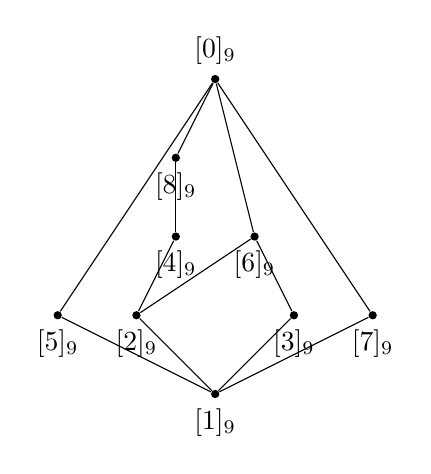
\begin{tikzpicture}
			\node[circle,fill=black,inner sep=0pt,minimum size=3pt,label=below:{$[1]_{9}$}](1) at (0,0){};
			\node[circle,fill=black,inner sep=0pt,minimum size=3pt,label=below:{$[5]_{9}$}](5) at (-2,1){};
			\node[circle,fill=black,inner sep=0pt,minimum size=3pt,label=below:{$[3]_{9}$}](3) at (1,1){};
			\node[circle,fill=black,inner sep=0pt,minimum size=3pt,label=below:{$[4]_{9}$}](4) at (-0.5,2){};
			\node[circle,fill=black,inner sep=0pt,minimum size=3pt,label=below:{$[2]_{9}$}](2) at (-1,1){};
			\node[circle,fill=black,inner sep=0pt,minimum size=3pt,label=below:{$[6]_{9}$}](6) at (0.5,2){};
			\node[circle,fill=black,inner sep=0pt,minimum size=3pt,label=below:{$[7]_{9}$}](7) at (2,1){};
			\node[circle,fill=black,inner sep=0pt,minimum size=3pt,label=below:{$[8]_{9}$}](8) at (-0.5,3){};
			\node[circle,fill=black,inner sep=0pt,minimum size=3pt,label=above:{$[0]_{9}$}](0) at (0,4){};
			\draw[thin,black] (1)--(5);
			\draw[thin,black] (1)--(2);
			\draw[thin,black] (1)--(3);
			\draw[thin,black] (1)--(7);
			\draw[thin,black] (2)--(4);
			\draw[thin,black] (2)--(6);
			\draw[thin,black] (3)--(6);
			\draw[thin,black] (4)--(8);
			\draw[thin,black] (5)--(0);
			\draw[thin,black] (8)--(0);
			\draw[thin,black] (6)--(0);
			\draw[thin,black] (7)--(0);
		\end{tikzpicture}
	\end{center}
Portandoci su $(\mathbb{Z},\rho)$ osserviamo che ogni classe di resto contiene infiniti interi:
\begin{align*}
	[n]_{9} = \{ z \in \mathbb{Z} \; | \; \exists k \in \mathbb{Z}(z = 9k +n)\}
\end{align*}
Dal diagramma di Hasse disegnato si osserva che gli interi appartenenti alla classe di 1 modulo 9 risultano essere minimali in $(\mathbb{Z},\rho)$. Analogamente, gli interi appartenenti alla classe di 0 modulo 9 (i multipli di 9) risultano essere massimali in $(\mathbb{Z},\rho)$. Poiché due elementi appartenenti alla stessa classe sono in relazione $\rho$ se e solo se essi coincidono abbiamo che due elementi distinti nella stessa classe di resto risultano essere inconfrontabili e quindi non esiste un minimo ed un massimo in $(\mathbb{Z},\rho)$.
\item Osserviamo che sia $127 \in [1]_{9}$ che $721 \in [1]_{9}$\footnote{Basta applicare i criteri di divisibilità.}. Quindi i due elementi sono inconfrontabili, essendo $[1]_{9}$ il minimo in $(\mathbb{Z}_{9},\divides)$ non esistono minoranti di $\{127,721\}$ mentre esistono infiniti interi, a due a due inconfrontabili, maggioranti di $\{127,721\}$, quindi non esiste neanche un estremo superiore.
\item Per i motivi esposti al punto precedente $(\mathbb{Z},\rho)$ non risulta essere un reticolo.
\item Osservando il diagramma di Hasse di $(\mathbb{Z}_{9},\divides)$ osserviamo che è possibile individuare una catena massimale considerando le classi $[1]_{9}, \ [2]_{9}, \ [4]_{9}, \ [8]_{9}, \ [0]_{9}$. Spostandoci in $(\mathbb{Z},\rho)$ e prendendo un singolo elemento di ciascuna classe si ottiene un sottoinsieme massimale (rispetto all'inclusione). Ad esempio:
\begin{displaymath}
	\{10,11,13,17,18\}
\end{displaymath}
\item Abbiamo:
\begin{itemize}
	\item $-90 \in [0]_{9}$
	\item $-15 \in [3]_{9}$
	\item $-3 \in [6]_{9}$
	\item $7 \in [7]_{9}$
	\item $15 \in [6]_{9}$
	\item $94 \in [4]_{9}$
	\item $100 \in [1]_{9}$
\end{itemize}
Otteniamo così il seguente diagramma di Hasse:
\begin{center}
	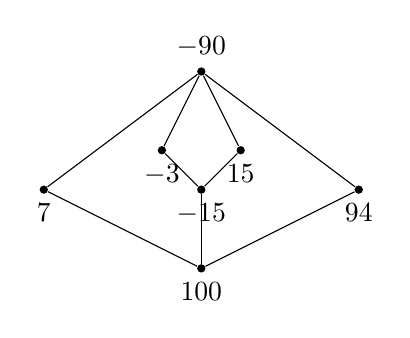
\begin{tikzpicture}
		\node[circle,fill=black,inner sep=0pt,minimum size=3pt,label=below:{$100$}](a) at (0,0){};
		\node[circle,fill=black,inner sep=0pt,minimum size=3pt,label=below:{$7$}](b) at (-2,1){};
		\node[circle,fill=black,inner sep=0pt,minimum size=3pt,label=below:{$-15$}](c) at (0,1){};
		\node[circle,fill=black,inner sep=0pt,minimum size=3pt,label=below:{$94$}](d) at (2,1){};
		\node[circle,fill=black,inner sep=0pt,minimum size=3pt,label=below:{$15$}](e) at (0.5,1.5){};
		\node[circle,fill=black,inner sep=0pt,minimum size=3pt,label=below:{$-3$}](f) at (-0.5,1.5){};
		\node[circle,fill=black,inner sep=0pt,minimum size=3pt,label=above:{$-90$}](g) at (0,2.5){};
		\draw[thin,black] (a)--(b);
		\draw[thin,black] (a)--(c);
		\draw[thin,black] (a)--(d);
		\draw[thin,black] (c)--(e);
		\draw[thin,black] (c)--(f);
		\draw[thin,black] (d)--(g);
		\draw[thin,black] (b)--(g);
		\draw[thin,black] (e)--(g);
		\draw[thin,black] (f)--(g);
	\end{tikzpicture}
\end{center}
Tale insieme ordinato è un reticolo complementato, ma non è distributivo in quanto il sottoreticolo: $$(\{100,7,-15,94,-90\},\rho)$$ è isomorfo al reticolo trirettangolo:
\begin{center}
	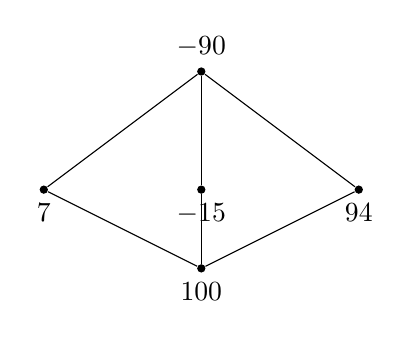
\begin{tikzpicture}
		\node[circle,fill=black,inner sep=0pt,minimum size=3pt,label=below:{$100$}](a) at (0,0){};
		\node[circle,fill=black,inner sep=0pt,minimum size=3pt,label=below:{$7$}](b) at (-2,1){};
		\node[circle,fill=black,inner sep=0pt,minimum size=3pt,label=below:{$-15$}](c) at (0,1){};
		\node[circle,fill=black,inner sep=0pt,minimum size=3pt,label=below:{$94$}](d) at (2,1){};
		\node[circle,fill=black,inner sep=0pt,minimum size=3pt,label=above:{$-90$}](g) at (0,2.5){};
		\draw[thin,black] (a)--(b);
		\draw[thin,black] (a)--(c);
		\draw[thin,black] (a)--(d);
		\draw[thin,black] (c)--(g);
		\draw[thin,black] (d)--(g);
		\draw[thin,black] (b)--(g);
	\end{tikzpicture}
\end{center}
\end{enumerate}
\subsection*{Esercizio 4}
\begin{enumerate}[label=(\textit{\roman*})]
	\item L'operazione $\ast$ risulta essere associativa e commutativa. Infatti:
	\begin{align*}
		\forall x,y \in \mathbb{Z}_{16} \bigl( x \ast y = 3xy = 3yx = y \ast x \bigr)
	\end{align*}
Inoltre, presi $a,b,c \in \mathbb{Z}_{16}$ abbiamo:
\begin{align*}
	a \ast (b \ast c ) = a \ast (3bc) = 3a(3bc) = 9abc \\
	(a \ast b) \ast c = (3ab) \ast c = 3(3ab)c = 9abc
\end{align*}
Un elemento $t \in \mathbb{Z}_{16}$ è neutro in $(\mathbb{Z}_{16},\ast)$ se e solo se, per ogni $a \in \mathbb{Z}_{16}$ risulta:
\begin{align*}
	a \ast t = t \ast a  = 3ta = a &\iff 3t \equiv_{16} 1 \\
	&\iff t = \overline{11}
\end{align*}
Quindi $t= \overline{11}$ è il neutro del monoide $(\mathbb{Z}_{16},\ast)$. Un elemento $a \in \mathbb{Z}_{16}$ ammette simmetrico se e solo se esiste un $a' \in \mathbb{Z}_{16}$ tale che $a \ast a' = 11$, ovvero:
\begin{align*}
	3aa' \equiv_{16} 11 &\iff aa' \equiv_{16} 9 & \text{\textcolor{gray}{(Moltiplicando per 11 inverso di 3)}}
\end{align*}
Tale equazione ammette soluzione se e solo se $(a,16) \divides 9$. I divisori di $16$ minori di 9 sono $1, \ 2, \ 4, \ 8$ e solo divide 9. Possiamo concludere che se $a \in \{1,3,5,7,9\}$ allora $(a,16)=1 \divides 9$. Troviamo l'inverso di $x=\overline{1}$:
\begin{align*}
	x \ast x' \equiv_{16} 11 &\iff 3x' \equiv_{16} 11 \\
	&\iff x' \equiv_{16} 9
\end{align*}
	\item Risulta $7 \ast 7 = 3 \cdot 49 = 3 \cdot 1 = 3 \notin H$, quindi $H$ non è stabile in $(\mathbb{Z}_{16},\ast)$
	\item Un elemento $a \in \mathbb{Z}_{16}$ è divisore dello zero in $(\mathbb{Z}_{16},+,\ast)$ se esiste un elemento $b \in \mathbb{Z}_{16} \setminus \{\overline{0}\}$ tale che $ a \ast b=\overline{0}$. Abbiamo:
	\begin{align*}
		a \ast b = 3ab = \overline{0}
	\end{align*}
Essendo $3$ coprimo con $16$ abbiamo che tale elemento è simmetrizzabile e quindi cancellabile, per rendere il prodotto nullo abbiamo quindi bisogno che $ab = \overline{0}$. Tale richiesta si traduce quindi nella ricerca dei divisori dello zero in $(\mathbb{Z}_{16},\cdot)$ i quali sono tutti e soli gli elementi non invertibili, cioè $\mathbb{Z}_{16} \setminus \mathcal{U}(\mathbb{Z}_{16}) = \{0,2,4,6,8,10,12,14\}$.
\end{enumerate}
\subsection*{Esercizio 5}
Un circuito euleriano in un grafo è un percorso chiuso che attraversa ciascun arco del grafo esattamente una volta. Perché un grafo possa ammettere un circuito euleriano, deve soddisfare due condizioni:
\begin{itemize}
	\item Tutti i vertici devono avere grado pari
	\item Il grafo deve essere connesso
\end{itemize}
Un grafo completo $K_{n}$​ è un grafo in cui ogni coppia di vertici è connessa da un arco, quindi in particolare è un grafo connesso. Per un grafo completo, il grado di ogni vertice è $n−1$, poiché ogni vertice è collegato a tutti gli altri $n−1$ vertici. Quindi se $n-1$ deve essere pari ciò significa che $n$ è un numero dispari. Quindi ogni grafo completo con un numero dispari di vertici ammette circuiti euleriani.
\subsection*{Esercizio 6}
\begin{enumerate}[label=(\textit{\roman*})]
	\item Applicando il Criterio di Eisenstein con $p=2$ abbiamo che $2$ divide i coefficienti $a_{0},...,a_{3}$, 2 non divide $a_{n}=4$ e $p^{2}=4$ non divide 2. Quindi il polinomio $f$ è irriducibile in $\mathbb{Q}$ e di conseguenza, essendo associato al polinomio $f_{1} \in \mathbb{Z}_{1}[x] = \mathbb{Z}[x]$, è irriducibile anche in $\mathbb{Z}[x]$.
	\item Risulta $f_{5} = 4x+2$. Per trovare un polinomio monico associato risolviamo l'equazione $4x \equiv{5} 1$ che ha soluzione per $x=4$, quindi moltiplicando $f_{5}$ per 4 otteniamo:
	\begin{align*}
		4 \cdot f_{5} &= 4 \cdot (4x+2)   \\
		&= 16x + 8 \\
		&= x + 3
	\end{align*}
Analogamente, per $f_{32}$ risolviamo l'equazione $5x \equiv_{32} 1$ ottenendo $x=13$. Moltiplichiamo quindi $f_{32}$ per $x=\overline{13}$:
\begin{align*}
	13 \cdot f_{32} &= 13 \cdot \bigl(5x^{4} + 10x^{2}+4x+2\bigr) \\
	&= x^{4} +2x^{2} +20x + 26
\end{align*}
\item Un polinomio è cancellabile se e solo se $cd(f)$ è cancellabile nell'anello dei coefficienti. In questo caso, essendo $cd(f)=5$ un numero primo abbiamo che per ogni intero non nullo $n <10$ 5 è coprimo con $n$ e quindi simmetrizzabile, quindi cancellabile.
\end{enumerate}
\vfill
\section{Esame del 13 luglio 2023}
\begin{center}
	\includegraphics[scale=.85]{pdf/23-07-13.pdf}
\end{center}
\subsection*{Esercizio 1}
Abbiamo:
\begin{enumerate}[label=(\textit{\roman*})]
	\item \textbf{Falso}. L'insieme vuoto non è un elemento del singleton del singleton dell'insieme vuoto ma è tutt'al più una sua parte.
	\item \textbf{Falso}. Non ha senso confrontare un numero cardinale con un insieme. Il simbolo $|\mathbb{N}|$ indica infatti la cardinalità di $\mathbb{N}$, ovvero il numero dei suoi elementi, che è quantificabile col simbolo $\aleph$. Il simbolo $\{\mathbb{N}\}$ indica invece il singleton dell'insieme dei numeri naturali.
	\item \textbf{Vera}. Notiamo infatti che l'antecedente risulta essere una proposizione falsa in quanto l'insieme dei tre elementi $\{1,2,3\}$ non è uguale all'insieme $\{3!\}=\{6\}$. L'implicazione risulta quindi essere vera in quanto l'antecedente è falsa.
	\item \textbf{Vera}. Una applicazione $f: \{1,2\} \rightarrow \mathbb{N}$ è un'applicazione per la quale $\forall x \in \{1,2\}$  esiste un $n \in \mathbb{N}$ tale che $n=f(x)$. Il grafico $\{(1,1),(2,1)\}$ descrive in particolare l'applicazione costante $c_{1}$ che associa l'elemento 1 ad ogni elemento dell'insieme $\{1,2\}$.
\end{enumerate}
\subsection*{Esercizio 2}
L'insieme $S = \mathbb{N} \cap [0]_{3}$ è l'insieme dei multipli di $3$, ovvero:
\begin{align*}
	S =  \mathbb{N} \cap [0]_{3} = \{n \in \mathbb{N} \; | \; \exists k \in \mathbb{N} (n=3k)\} = 3\mathbb{N}
\end{align*}
L'applicazione caratteristica $\text{\Large\chi}_{\mathbb{N},S}$ restituisce 1 se $n \in 3\mathbb{N}$, 0 altrimenti. In particolare, $\forall n \in \mathbb{N}$:
\begin{align}\label{eq:130723_20}
	n^{\chi(a)} = 
	\begin{cases}
		a^{1} &\iff a \in 3\mathbb{N} \\
		a^{0} &\iff a \notin 3\mathbb{N}
	\end{cases}
\end{align}
\begin{enumerate}[label=(\textit{\roman*})]
	\item L'operazione $\ast$ è banalmente commutativa in quanto lo è la moltiplicazione ordinaria in $\mathbb{N}$. Per verificare l'associatività bisogna verificare che per ogni terna numerica $(a,b,c)$ di elementi di $\mathbb{N}$ risulti:
	\begin{align*}
		(a \ast b) \ast c = a \ast (b \ast c)
	\end{align*}
	Sviluppando il membro a sinistra otteniamo:
	\begin{align}
		(a \ast b) \ast c &= \bigl(a^{\chi(a)} \cdot b^{\chi(b)} \bigr) \ast c \nonumber \\
		&= \bigl( a^{\chi(a)} \cdot b^{\chi(b)}\bigr)^{\chi(a^{\chi(a)} \cdot b^{\chi(b)})} \cdot c^{\chi(c)} \label{eq:130723_21}
	\end{align}
	Mentre, sviluppando il membro a destra:
	\begin{align}
		a \ast (b \ast c) &= (b \ast c) \ast a & \text{\textcolor{gray}{(Applicando la commutatività di $\ast$)}} \nonumber \\
		&= \bigl(b^{\chi(b)}\cdot c^{\chi(c)}\bigr)^{\chi(b^{\chi(b)} \cdot c^{\chi(c)})} \cdot a^{\chi(a)} \label{eq:130723_22}
	\end{align}
	La verifica dell'uguaglianza di \ref{eq:130723_21} con \ref{eq:130723_22} deve essere fatta per casi:
	\begin{enumerate}
		\item Supponiamo il caso in cui $a,b,c \in 3\mathbb{N}$, in questo caso, applicando quanto osservato in \ref{eq:130723_20} otteniamo:
		\begin{align*}
			(a \ast b) \ast c &= \bigl( a^{\chi(a)} \cdot b^{\chi(b)}\bigr)^{\chi(a^{\chi(a)} \cdot b^{\chi(b)})} \cdot c^{\chi(c)} & \text{\textcolor{gray}{
					(Osservando che $ab \in 3\mathbb{N}$)}}\\
			&= (a\cdot b) \cdot c = (ab)c 
		\end{align*}
		e analogamente:
		\begin{align*}
			a \ast (b \ast c) &= \bigl(b^{\chi(b)}\cdot c^{\chi(c)}\bigr)^{\chi(b^{\chi(b)} \cdot c^{\chi(c)})} \cdot a^{\chi(a)} \\
			&= (b \cdot c) \cdot a = a(bc)
		\end{align*}
		\item Siano ora $a,b,c \notin 3\mathbb{N}$. Allora:
		\begin{align*}
			(a \ast b) \ast c = (1 \cdot 1)^{0} \cdot 1 = 1 \\
			(a \ast b) \ast c =  (1 \cdot 1)^{0} \cdot 1 = 1
		\end{align*}
		\item Sia uno tra $a,b,c$ non appartenente a $3\mathbb{N}$. Senza ledere di generalità, sia esso $c$. Abbiamo quindi:
		\begin{align*}
			(a \ast b) \ast c = (a \cdot b) ^{1} \cdot 1 = ab \\
			a \ast (b \ast c) = a(b \cdot 1)^{1} = ab
		\end{align*}
		\item Siano due elementi non appartenenti a $3\mathbb{N}$, siano essi $b,c$, allora:
		\begin{align*}
			(a \ast b) \ast c = (a \cdot 1)^{1} = a \\
			a \ast (b \ast c) = a \cdot (1 \cdot 1)^{0} = a
		\end{align*}
	\end{enumerate}
	In ogni caso il membro a destra e a sinistra coincidono e quindi $\ast$ risulta associativa.
	\item Per esistere elemento neutro rispetto all'operazione $\ast$ deve esistere un $t \in \mathbb{N}$ tale che, per ogni $n \in \mathbb{N}$, garantisca che $n \ast t = t \ast n = n$. Un tale $t$ non può esistere in quanto:
	\begin{align*}
		\forall n \in \mathbb{N} \bigl(n \ast t = n &\iff n^{\chi(n)} \cdot t^{\chi(t)} = n \\
		&\iff n^{\chi(n)} = n \land t^{\chi(t)}=1 \\
		&\iff (n \in 3\mathbb{N}) \land (t \notin 3\mathbb{N}) \bigr)
	\end{align*}
	Dato che non può esistere un tale $t$ che sia neutro per ogni naturale possiamo concludere affermando la sua non esistenza.
	\item Abbiamo $T=2\mathbb{N}$ e $U=\{n \in \mathbb{N} \; | \; \exists k \in \mathbb{N}(n=3k+2)\}$. Una parte $X \subseteq \mathbb{N}$ si dice stabile se, e solo se, per ogni $(a,b) \in X \times X$ si abbia $a \ast b \in X$.
	\begin{itemize}
		\item Presi ad esempio $a=14$ e $b=16$ elementi di $T$ abbiamo:
		\begin{align*}
			14 \ast 16 &= 14^{\chi(14)} \cdot 16^{\chi(16)} \\
			&= 14^{0} \cdot 16^{0} = 1 \notin T
		\end{align*}
		Quindi $T$ non è stabile.
		\item Presi $a=5$ e $b=7$ elementi di $U$, abbiamo:
		\begin{align*}
			5 \ast 7 &= 5^{\chi(5)} \cdot 7^{\chi(7)} \\
			&= 1 \notin U
		\end{align*}
		Quindi $U$ non è stabile.
		\item Presi due elementi $a,b \in S$ abbiamo:
		\begin{align*}
			a \ast b = a^{\chi(a)} \cdot b^{\chi(b)} \\
			&= a \cdot b \in S
		\end{align*}
		Quindi il semigruppo $(S,\ast)$ risulta stabile rispetto a $\ast$.
	\end{itemize}
\end{enumerate}
\subsection*{Esercizio 3}
\begin{enumerate}[label=(\textit{\roman*})]
	\item La relazione $\alpha$ coincide con la relazione identica $id_{\mathbb{N}}$ che è una relazione d'ordine. In $(\mathbb{N},\alpha)$ tutti i numeri sono sia minimali che massimali. Non esistono minimo e massimo. Non potendo definire, per ogni coppia di elementi $(n,m)$ l'infimo ed il supremo della parte $\{a,b\}$ l'insieme ordinato non costituisce un reticolo.
	Presa la parte $S=\{1,20,40,400,10000\}$ abbiamo il seguente diagramma di Hasse:
	\begin{center}
		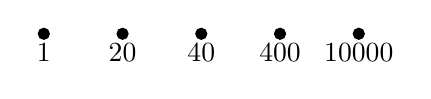
\begin{tikzpicture}
			\filldraw[black] (0,0) circle(2pt) node[anchor=north]{1};
			\filldraw[black] (1,0) circle(2pt) node[anchor=north]{20};
			\filldraw[black] (2,0) circle(2pt) node[anchor=north]{40};
			\filldraw[black] (3,0) circle(2pt) node[anchor=north]{400};
			\filldraw[black] (4,0) circle(2pt) node[anchor=north]{10000};
		\end{tikzpicture}
	\end{center}
	\item  Per verificare che $\beta \in OL(\mathbb{N})$ verifichiamo che essa sia riflessiva, antisimmetrica e transitiva:
	\begin{enumerate}
		\item Chiaramente $\forall a \in \mathbb{N}$ risulta $a \ \beta \ a $ in quanto $a=a$ e questo è sufficiente per garantire la corrispondenza di un numero con se stesso.
		\item Siano $a,b \in \mathbb{N}$ tali che $a \ \beta \ b$ e $b \ \beta \ a$:
		\begin{align}
			\begin{cases}
				a \ \beta \ b &\iff a=b \lor (a \divides b \land a < 10b) \\
				b \ \beta \ a &\iff b=a \lor (b \divides a \land b < 10a)
			\end{cases}
		\end{align}
		Nel caso gli elementi coincidano l'antisimmetria di $\beta$ è una conseguenza triviale. Se $a \divides b \land a <10b$ e $b \divides a \land b<10a$ allora, in particolare, gli elementi risultano essere elementi associati in $\mathbb{N}$ e quindi devono coincidere per forza.
		\item Siano $a,b,c \in \mathbb{N}$ elementi tali che $a \ \beta \ b$ e $b \ \beta \ c$. Allora, se $a=b$ e $b=c$ allora $a=c$ e quindi $ a \ \beta \ c$. Altrimenti, se $a \divides b \land a <10b$ e $b \divides c \land b<10c$ allora possiamo scrivere $b=ka$ per un opportuno $k \in \mathbb{N}$ e $c=mb=m(ka)=a(km)$. Quindi $a \divides c$ e inoltre possiamo eseguire la maggiorazione $a < 10b < 100c$. Quindi vale sicuramente $a < 10c$ e $a \ \beta \ c$. Quindi $\beta \in OL(\mathbb{N})$.	
	\end{enumerate}
	L'elemento 1 risulta essere il minimo in $(\mathbb{N},\beta)$ in quanto, $\forall n \in \mathbb{N}(1 \ \beta \ n)$. Dato che per ogni $a,b$ esiste sempre un elemento $n \in \mathbb{N}$ tale che $n \cdot a > b$, possiamo dire che in  $(\mathbb{N},\beta)$ non esistono elementi massimali e dunque un massimo. L'insieme ordinato risulta essere un reticolo in quanto per ogni parte $\{a,b\}$ possiamo trovare l'infimo ed il supremo che è dato dal massimo comun divisore e dal minimo comune multiplo di $(a,b)$. In particolare $(S,\beta)$ risulta essere un insieme totalmente ordinato. Si ottiene quindi la catena:
	\begin{center}
		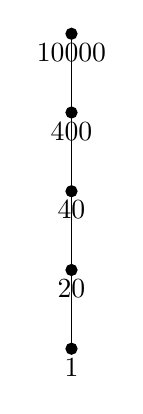
\begin{tikzpicture}
			\filldraw[black] (0,0) circle(2pt) node[anchor=north]{1};
			\filldraw[black] (0,1) circle(2pt) node[anchor=north]{20};
			\filldraw[black] (0,2) circle(2pt) node[anchor=north]{40};
			\filldraw[black] (0,3) circle(2pt) node[anchor=north]{400};
			\filldraw[black] (0,4) circle(2pt) node[anchor=north]{10000};
			\draw[black](0,0)--(0,1)--(0,2)--(0,3)--(0,4);
		\end{tikzpicture}
	\end{center}
	\item La relazione $\gamma$ coincide con la relazione $\alpha$ in quanto osserviamo che la proposizione $(a \divides b \land a > 10b)$ risulta sempre falsa. Infatti un divisore non può essere maggiore di un multiplo dell'elemento che divide. Resta però la condizione di uguaglianza la quale, come visto nel primo punto, risulta essere una relazione d'ordine.
	\item La relazione $\delta$ non risulta essere una relazione d'ordine in $\mathbb{N}$ in quanto non soddisfa la proprietà antisimmetrica. Infatti presi $a,b \in \mathbb{N}$ tali che $a \ndivides b$ e $b \ndivides a$, ovvero $a \ \delta \ b$ e $b \ \delta \ a$, ciò non implica che sia necessariamente $a=b$. Ad esempio abbiamo $2 \ \delta \ 5$ e $5 \ \delta \ 2$ in quanto $2 \ndivides 5$ e $5 \ndivides 2$ ma $2 \neq 5$.
\end{enumerate}

\subsection*{Esercizio 4}
Un grafo si dice connesso se per ogni coppia di vertici esiste un cammino. Se il numero di vertici è pari a 16 ciò significa che devono esistere almeno 15 lati. Per questo motivo non è possibile disegnare un grafo connesso con 16 vertici e 10 lati.
\subsection*{Esercizio 5}
Calcoliamo il Massimo Comun Divisore tra 111 e 126.
\begin{align*}
	111 = 3 \cdot 37 \\
	126 = 2 \cdot 3^{2} \cdot 7
\end{align*}
L'equazione $111n \equiv_{126} 11$ non ammette soluzioni in quanto $MCD(111,126)=3$ non divide 11, mentre $111n \equiv_{126} 12$ risulta essere una equazione compatibile. Dividendo tutti i termini per 3 si ottiene l'equazione equivalente ridotta:
\begin{align*}
	\frac{111}{3}n \equiv_{\frac{126}{3}} \frac{12}{3} = 37n \equiv_{42} 4
\end{align*}
E vale $MCD(37,42)=1$. Cerchiamo una combinazione lineare $37u+42v=1$. Applicando l'algoritmo delle divisioni successive si ottiene:
\begin{align*}
	42 = 37 \cdot 1 + 5 \\
	37 = 5 \cdot 7 + 2 \\
	5 = 2 \cdot 2 + 1 \\
	2 = 1 \cdot 2 + 0
\end{align*}
Da queste relazioni otteniamo:
\begin{align}
	5 = 42 +(-1)37 \\
	2 = 37 +(-7)5 \\
	1 = 5 + (-2)2
\end{align}
Possiamo dunque esprimere 1 come:
\begin{align*}
	1 &= 5 - 4 \\
	&= \bigl(42-37\bigr)+(-2)\bigl(37-35\bigr) \\
	&= 42 - 37 +(-2)37+(14)5 \\
	&= 42+ (-3)37 +(14)\bigl(42+(-1)37\bigr) \\
	&= 42 + (-3)37 + (14)42+(-14)37 \\
	&= (15)42 + (-17)37
\end{align*}
Moltiplicando tale combinazione lineare per 4 si ottiene:
\begin{align*}
	4 = (60)42 + (-68)37
\end{align*}
Quindi $u=[-68]_{42}=[16]_{42}$ è soluzione dell'equazione. L'insieme $A=\{[16]_{42}\}$ e vale $\{a \in A \; | \; 0 \leq a \leq 84\} = \{16,58\}$.
\subsection*{Esercizio 6}
\begin{enumerate}[label=(\textit{\roman*})]
	\item L'insieme $S$ è costituito dai polinomi $f \in \mathbb{Z}_{5}$ di grado 4 tali che $f(\overline{1})=0$. Un polinomio di grado 4 in $\mathbb{Z}_{5}[x]$ può essere scritto come:
	\begin{align*}
		a_{4}x^{4}+a_{3}x^{3}+a_{2}x^{2}+a_{1}x+a_{0}
	\end{align*}
	Con $a_{4} \neq \overline{0}$, altrimenti non sarebbe un polinomio di quarto grado. Imporre che $f(\overline{1})=0$ è equivalente a dire che:
	\begin{align*}
		a_{4}+a_{3}+a_{2}+a_{1}+a_{0} = 0
	\end{align*}
	La domanda della conta degli elementi di $S$ può essere rivista come il conteggio di tutte le possibili combinazioni degli elementi $a_{i}$ con $i \in \mathbb{Z}_{5}$ tali che $\sum_{i=0}^{4} a_{i}=0$ e tale che $a_{4} \neq \overline{0}$.
	Per ciascuno di questi casi, stiamo essenzialmente chiedendo in quanti modi possiamo scegliere $4$ numeri da $\{0, 1, 2, 3, 4\}$ la cui somma sia un valore specifico. Abbiamo quindi:
	\begin{itemize}
		\item Se $a_{4}=1$, deve essere $a_{3}+a_{2}+a_{1}+a_{0}=4$;
		\item Se $a_{4}=2$, deve essere $a_{3}+a_{2}+a_{1}+a_{0}=3$;
		\item Se $a_{4}=3$, deve essere $a_{3}+a_{2}+a_{1}+a_{0}=2$;
		\item Se $a_{4}=4$, deve essere $a_{3}+a_{2}+a_{1}+a_{0}=1$.
	\end{itemize}
	Per ogni caso, il numero di combinazioni con ripetizione di $4$ elementi presi dall'insieme $\mathbb{Z}_{5}$ che diano somma $k$ con $k \in \{4,3,2,1\}$ è dato da:
	\begin{align*}
		\sum_{k=1}^{4} \binom{4+k-1}{i} &= \binom{4+1-1}{1}+\binom{4+2-1}{2}+\binom{4+3-1}{3}+\binom{4+4-1}{4} \\
		&= 4 + 10 + 20 + 35 \\
		&= 69
	\end{align*}
	\item $(S,+)$ è una parte chiusa. Infatti, presi due polinomi $s,q \in S$ allora $s+q$ calcolato in $\overline{1}$ è equivalente a $s(1)+q(1)=0$. $(S,+)$ non risulta essere abeliano in quanto il polinomio nullo non è un polinomio di grado 4.
	\item Osserviamo che per ogni $f \in S\bigl(\varphi(f)= f(\overline{1})=\overline{0}\bigr)$, e $\varphi$ risulta essere una applicazione costante. Quindi $\varphi$ non è iniettiva e non è suriettiva. 
	\item Essendo costante $\varphi$ il suo nucleo di equivalenza coincide con la relazione totale in $S$. Quindi $S/{\sim_{\varphi}} = S/{\tau_{S}} = \{S\}$, ed esiste un'unica classe di equivalenza.
\end{enumerate}
\vfill
